\documentclass[11pt,a4paper,oneside]{report}             % Single-side
%\documentclass[11pt,a4paper,twoside,openright]{report}  % Duplex

%\PassOptionsToPackage{chapternumber=Huordinal}{magyar.ldf}
\usepackage{t1enc}
\usepackage[latin2]{inputenc}
\usepackage{amsmath}
\usepackage{amssymb}
\usepackage{enumerate}
\usepackage[thmmarks]{ntheorem}
\usepackage{graphics}
\usepackage{epsfig}
\usepackage{listings}
\usepackage{color}
%\usepackage{fancyhdr}
\usepackage{lastpage}
\usepackage{anysize}
\usepackage[magyar]{babel}
\usepackage{sectsty}
\usepackage{setspace}  % Ettol a tablazatok, abrak, labjegyzetek maradnak 1-es sorkozzel!
\usepackage[hang]{caption}
\usepackage{hyperref}

%--------------------------------------------------------------------------------------
% Main variables
%--------------------------------------------------------------------------------------
\newcommand{\vikszerzo}{Balogh T�mea}
\newcommand{\vikkonzulens}{Debreceni Csaba}
\newcommand{\vikcim}{Modellelemek effekt�v jogosults�gainak sz�rmaztat�sa finomszemcs�s hozz�f�r�si szab�lyokb�l}
\newcommand{\viktanszek}{M�r�stechnika �s Inform�ci�s Rendszerek Tansz�k}
\newcommand{\vikdoktipus}{Szakdolgozat}
\newcommand{\vikdepartmentr}{Balogh T�mea}

%--------------------------------------------------------------------------------------
% Page layout setup
%--------------------------------------------------------------------------------------
% we need to redefine the pagestyle plain
% another possibility is to use the body of this command without \fancypagestyle
% and use \pagestyle{fancy} but in that case the special pages
% (like the ToC, the References, and the Chapter pages)remain in plane style

\pagestyle{plain}
%\setlength{\parindent}{0pt} % �ttekinthet�bb, angol nyelv� dokumentumokban jellemz�
%\setlength{\parskip}{8pt plus 3pt minus 3pt} % �ttekinthet�bb, angol nyelv� dokumentumokban jellemz�
\setlength{\parindent}{12pt} % magyar nyelv� dokumentumokban jellemz�
\setlength{\parskip}{0pt}    % magyar nyelv� dokumentumokban jellemz�

\marginsize{35mm}{25mm}{15mm}{15mm} % anysize package
\setcounter{secnumdepth}{0}
\sectionfont{\large\upshape\bfseries}
\setcounter{secnumdepth}{2}
\singlespacing
\frenchspacing

%--------------------------------------------------------------------------------------
%	Setup hyperref package
%--------------------------------------------------------------------------------------
\hypersetup{
    bookmarks=true,            % show bookmarks bar?
    unicode=false,             % non-Latin characters in Acrobat�s bookmarks
    pdftitle={\vikcim},        % title
    pdfauthor={\vikszerzo},    % author
    pdfsubject={\vikdoktipus}, % subject of the document
    pdfcreator={\vikszerzo},   % creator of the document
    pdfproducer={Producer},    % producer of the document
    pdfkeywords={keywords},    % list of keywords
    pdfnewwindow=true,         % links in new window
    colorlinks=true,           % false: boxed links; true: colored links
    linkcolor=black,           % color of internal links
    citecolor=black,           % color of links to bibliography
    filecolor=black,           % color of file links
    urlcolor=black             % color of external links
}

%--------------------------------------------------------------------------------------
% Set up listings
%--------------------------------------------------------------------------------------
\lstset{
	basicstyle=\scriptsize\ttfamily, % print whole listing small
	keywordstyle=\color{black}\bfseries\underbar, % underlined bold black keywords
	identifierstyle=, 					% nothing happens
	commentstyle=\color{white}, % white comments
	stringstyle=\scriptsize\sffamily, 			% typewriter type for strings
	showstringspaces=false,     % no special string spaces
	aboveskip=3pt,
	belowskip=3pt,
	columns=fixed,
	backgroundcolor=\color{lightgray},
} 		
\def\lstlistingname{lista}	

%--------------------------------------------------------------------------------------
%	Some new commands and declarations
%--------------------------------------------------------------------------------------
\newcommand{\code}[1]{{\upshape\ttfamily\scriptsize\indent #1}}

% define references
\newcommand{\figref}[1]{\ref{fig:#1}.}
\renewcommand{\eqref}[1]{(\ref{eq:#1})}
\newcommand{\listref}[1]{\ref{listing:#1}.}
\newcommand{\sectref}[1]{\ref{sect:#1}}
\newcommand{\tabref}[1]{\ref{tab:#1}.}

\DeclareMathOperator*{\argmax}{arg\,max}
%\DeclareMathOperator*[1]{\floor}{arg\,max}
\DeclareMathOperator{\sign}{sgn}
\DeclareMathOperator{\rot}{rot}
\definecolor{lightgray}{rgb}{0.95,0.95,0.95}

\author{\vikszerzo}
\title{\viktitle}
\includeonly{
	guideline,%
	project,%
	titlepage,%
	declaration,%
	abstract,%
	introduction,%
	chapter1,%
	chapter2,%
	chapter3,%
	chapter4,%
	chapter5,%
	chapter6,%
	summary,%
	acknowledgement,%
	appendices,%
}
%--------------------------------------------------------------------------------------
%	Setup captions
%--------------------------------------------------------------------------------------
\captionsetup[figure]{
%labelsep=none,
%font={footnotesize,it},
%justification=justified,
width=.75\textwidth,
aboveskip=10pt}

\renewcommand{\captionlabelfont}{\small\bf}
\renewcommand{\captionfont}{\footnotesize\it}

%--------------------------------------------------------------------------------------
% Table of contents and the main text
%--------------------------------------------------------------------------------------
\begin{document}
\singlespacing
%--------------------------------------------------------------------------------------
% Feladatkiiras (a tanszeken atveheto, kinyomtatott valtozat)
%--------------------------------------------------------------------------------------
\clearpage
\begin{center}
\large
\textbf{FELADATKI�R�S}\\
\end{center}

A feladatki�r�st a tansz�ki adminisztr�ci�ban lehet �tvenni, �s a leadott munk�ba eredeti, tansz�ki pecs�ttel ell�tott �s a tansz�kvezet� �ltal al��rt lapot kell belef�zni (ezen oldal \emph{helyett}, ez az oldal csak �tmutat�s). Az elektronikusan felt�lt�tt dolgozatban m�r nem kell beleszerkeszteni ezt a feladatki�r�st.





\pagenumbering{arabic}
\onehalfspacing
%--------------------------------------------------------------------------------------
%	The title page
%--------------------------------------------------------------------------------------
\begin{titlepage}
\begin{center}

\includegraphics[width=60mm,keepaspectratio]{src/figures/BMElogo.png}\\
\vspace{0.3cm}
\textbf{Budapesti M�szaki �s Gazdas�gtudom�nyi Egyetem}\\
\textmd{Villamosm�rn�ki �s Informatikai Kar}\\
\textmd{\viktanszek}\\[5cm]

\vspace{0.4cm}
{\huge \bfseries \vikcim}\\[0.8cm]
\vspace{0.5cm}
\textsc{\Large \vikdoktipus}\\[4cm]

\begin{tabular}{cc}
 \makebox[7cm]{\emph{K�sz�tette}} & \makebox[7cm]{\emph{Konzulens}} \\
 \makebox[7cm]{\vikszerzo} & \makebox[7cm]{\vikkonzulens}
\end{tabular}

\vfill
{\large \today}
\end{center}
\end{titlepage}



\tableofcontents\vfill
%--------------------------------------------------------------------------------------
% Nyilatkozat
%--------------------------------------------------------------------------------------
\begin{center}
\large
\textbf{HALLGAT�I NYILATKOZAT}\\
\end{center}

Alul�rott \emph{\vikszerzo}, szigorl� hallgat� kijelentem, hogy ezt a szakdolgozatot meg nem engedett seg�ts�g n�lk�l, saj�t magam k�sz�tettem, csak a megadott forr�sokat (szakirodalom, eszk�z�k stb.) haszn�ltam fel. Minden olyan r�szt, melyet sz� szerint, vagy azonos �rtelemben, de �tfogalmazva m�s forr�sb�l �tvettem, egy�rtelm�en, a forr�s megad�s�val megjel�ltem.

Hozz�j�rulok, hogy a jelen munk�m alapadatait (szerz�(k), c�m, angol �s magyar nyelv� tartalmi kivonat, k�sz�t�s �ve, konzulens(ek) neve) a BME VIK nyilv�nosan hozz�f�rhet� elektronikus form�ban, a munka teljes sz�veg�t pedig az egyetem bels� h�l�zat�n kereszt�l (vagy autentik�lt felhaszn�l�k sz�m�ra) k�zz�tegye. Kijelentem, hogy a beny�jtott munka �s annak elektronikus verzi�ja megegyezik. D�k�ni enged�llyel titkos�tott diplomatervek eset�n a dolgozat sz�vege csak 3 �v eltelte ut�n v�lik hozz�f�rhet�v�.

\begin{flushleft}
\vspace*{1cm}
Budapest, \today
\end{flushleft}

\begin{flushright}
 \vspace*{1cm}
 \makebox[7cm]{\rule{6cm}{.4pt}}\\
 \makebox[7cm]{\emph{\vikszerzo}}\\
 \makebox[7cm]{hallgat�}
\end{flushright}
\thispagestyle{empty}

\vfill
\clearpage
\thispagestyle{empty} % an empty page


%----------------------------------------------------------------------------
% Abstract in hungarian
%----------------------------------------------------------------------------
\chapter*{Kivonat}\addcontentsline{toc}{chapter}{Kivonat}

Bizonyos informatikai rendszerek �zemeltet�se eset�n a vel�k szemben t�masztott els�dleges k�vetelm�ny, hogy ne vesz�lyeztessenek emberi �leteket, ne okozzanak anyagi, term�szeti k�rokat. Ilyen �gynevezett biztons�gkritikus rendszerek p�ld�ul a vas�ti-, rep�l�g�p ir�ny�t�si berendez�sek, nukle�ris er�m�vek.

Komplexit�suk miatt ezek tradicion�lis k�d alap� fejleszt�s�t egyre ink�bb felv�ltja a modellvez�relt megk�zel�t�s, amely sor�n magasszint� modellekb�l kiindulva, azokat tov�bb finom�tva a rendszer a legapr�bb r�szletekig megtervezhet�. A metodika el�nyei t�bbek k�z�tt az automatikus k�d-, teszteset- �s dokument�ci�-gener�l�s, valamint, hogy a l�trej�v� modellek verifik�l�s�val m�r a fejleszt�s korai szakasz�ban kisz�rhet�k bizonyos hib�k.

Ezeken a komplex rendszereken �ltal�ban egy vagy ak�r t�bb c�g fejleszt� csapatai kollaborat�v m�don dolgoznak. �gy felmer�l a modellelemek biztons�g�nak k�rd�se is, legyen sz� olyan bizalmas adatr�l, l�trej�v� szellemi tulajdonr�l, amelyhez csak bizonyos poz�ci�kban l�v� felhaszn�l�k f�rhetnek hozz�, vagy a rendszernek olyan kritikus r�sz�r�l, amelyet csak megfelel� szaktud�ssal rendelkez� fejleszt�k m�dos�thatnak.

A MONDO nemzetk�zi kutat�si projektben k�sz�lt kollabor�ci�s keretrendszer modellszinten, finomszemcs�s szab�lyok alapj�n v�gzi a hozz�f�r�s-vez�rl�st. Ezekben a szab�lyokban gr�flek�rdez�sekkel hat�rozhat� meg, hogy a modellnek milyen t�pus� vagy pontosan mely elemeire milyen jogok vonatkozzanak k�l�nb�z� felhaszn�l�k tekintet�ben.

Munk�m sor�n sz�veges szintaxist defini�ltam a hozz�f�r�si szab�lyok meghat�roz�s�hoz, majd implement�ltam egy olyan algoritmust, amely k�pes ilyen szab�lyok EMF modellek feletti ki�rt�kel�s�re, vagyis az effekt�v �rv�nyre jut� hozz�f�r�sek kisz�m�t�s�ra. Az algoritmust a m�r eml�tett MONDO projekt egyik esettanulm�nyak�nt haszn�lt sz�lturbina vez�rl�r�l k�sz�lt modellel teszteltem. V�g�l az elk�sz�lt nyelvtan �s algoritmus integr�l�sra ker�lt a kollabor�ci�s keretrendszerbe.
\vfill

%----------------------------------------------------------------------------
% Abstract in english
%----------------------------------------------------------------------------
\chapter*{Abstract}\addcontentsline{toc}{chapter}{Abstract}


\vfill


%----------------------------------------------------------------------------
\chapter{Bevezet�s}
%----------------------------------------------------------------------------

A nagym�ret�, komplex ipari szoftverek fejleszt�se t�bb ember egy�ttes munk�j�t ig�nyli. A tervez�s modellalap� megk�zel�t�se az�rt is el�ny�s, mert a magasszint� modellek ak�r k�l�nb�z� szakter�leteken mozg� fejleszt� csapatok sz�m�ra is ugyanolyan m�don �rtelmezhet�k, ami el�seg�ti a hat�kony, �sszehangolt munkav�gz�st.

Ezen komplex modellek kollaborat�v fejleszt�se offline vagy online form�ban val�sul meg. El�bbi esetben a felhaszn�l�k egy k�z�s t�rhelyen l�v�, verzi�kezelt modellb�l k�rik le a saj�t p�ld�nyukat, majd a m�dos�t�sok v�grehajt�sa ut�n visszak�ldik azokat a szerverre. A t�bbiek csak akkor �rtes�lnek ezekr�l a v�ltoz�sokr�l, amikor friss�tik a saj�tjukat a k�z�s modell alapj�n. �gy, ha k�zben �k is dolgoztak rajta, akkor az �sszef�s�lend� verzi�k k�z�tt ad�dhatnak konfliktusok. Ezzel szemben online kollabor�ci� sor�n a felhaszn�l�k �ltal eszk�z�lt v�ltoz�sok mindenki sz�m�ra r�gt�n l�that�k a modellen.

Offline �s online forgat�k�nyv eset�n is felmer�l a modellelemek biztons�g�nak, hozz�f�r�s-szab�lyoz�snak a k�rd�se. Abban az esetben p�ld�ul, amikor egy c�g a munka egy bizonyos r�sz�t ledeleg�lja egy m�sik c�gnek, az adott modell megfelel� r�szeit el�rhet�v� teszi neki. Viszont lehetnek a modellnek bizalmas, a c�g szellemi tulajdon�nak sz�m�t� elemei, amelyekhez nem akar hozz�f�r�st biztos�tani az alv�llalkoz� sz�m�ra. Hasonl�an, ha p�ld�ul vannak a modellnek olyan kritikus r�szei, amelyek fejleszt�se speci�lis szaktud�st ig�nyel, akkor ezeket csak a hozz��rt� felhaszn�l�k m�dos�thatj�k, a t�bbiek nem f�rhetnek hozz�juk.

Modellek feletti hozz�f�r�s-kezel�sre l�tez� gyakorlat, hogy a modelleket, modellr�szeket tartalmaz� f�jlokhoz hat�roznak meg olvas�si, �r�si jogosults�gokat. A rendszert �jabb felhaszn�l�kkal, �s sz�mukra meghat�rozott hozz�f�r�si szab�lyokkal b�v�tve a modell megfelel� fragmenseit le kell v�lasztani, �s k�l�n f�jlban elt�rolni. Ezt a jelens�get szeml�lteti \aref{fig:filelevel} �bra, ennek hat�s�ra a modell elemek ezreire apr�z�dhat. A f�jlszint� szab�lyoz�s h�tr�nya, hogy ez a jelens�g a rendszert nehezen sk�l�zhat�v�, rugalmatlann� teszi.

\begin{figure}[tb]
	\begin{center}
		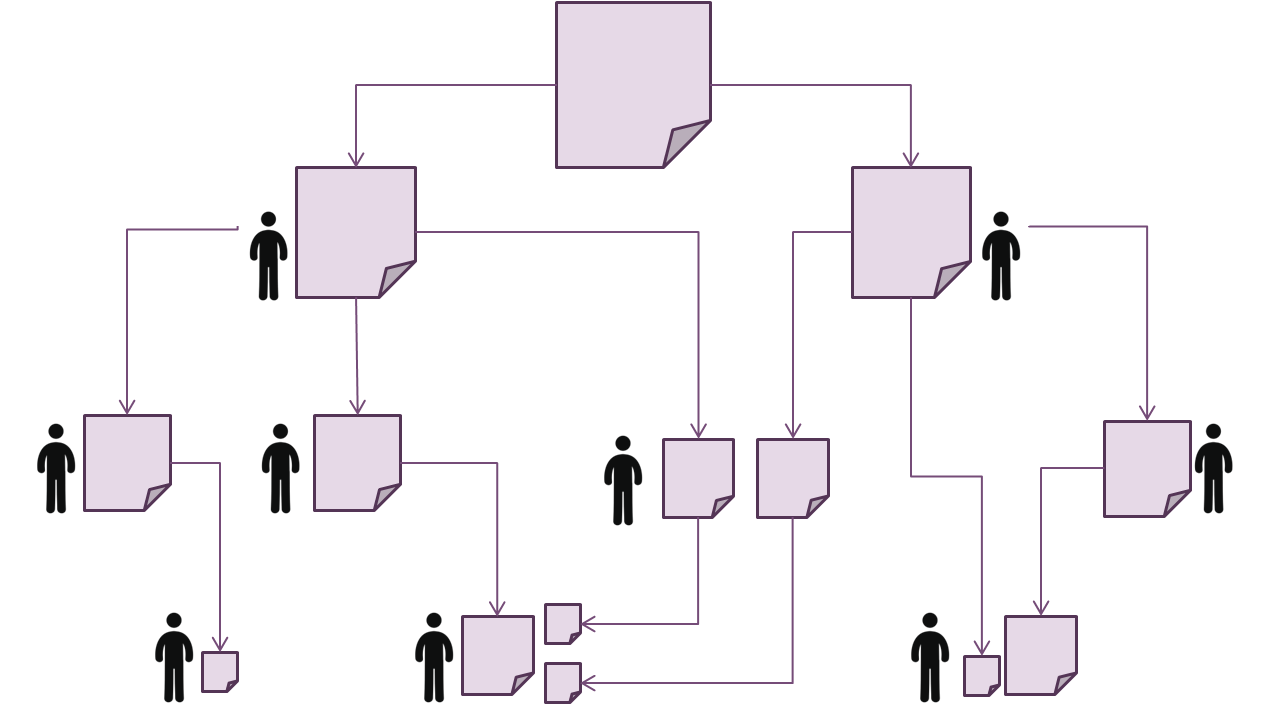
\includegraphics[width=.8\columnwidth]{src/figures/filelevel}
		\caption{A f�jlszint� hozz�f�r�s-szab�lyoz�s probl�m�ja}
		\label{fig:filelevel}
	\end{center}
\end{figure}

Erre a probl�m�ra a hozz�f�r�sek modellszint� szab�lyoz�sa ny�jt megold�st. A MONDO nemzetk�zi kutat�si projektben k�sz�lt kollabor�ci�s keretrendszer finomszemcs�s szab�lyok alapj�n v�gzi a hozz�f�r�s-vez�rl�st. Ezekben a modell elemi r�szeire, objektumokra �s azok attrib�tumaira, referenci�ira k�l�n-k�l�n lehet hozz�f�r�si jogokat meghat�rozni a k�l�nb�z� felhaszn�l�k tekintet�ben. A k�rd�ses modellelemeket gr�flek�rdez�s eredm�nyek�nt kapjuk, amely �gy is megfogalmazhat�, hogy tetsz�leges sz�m� �s tulajdons�g� elemet adjon vissza. �gy egy milli�s nagys�grend� modell eset�n nem sz�ks�ges egyes�vel minden egyes elemre le�rni a jogosults�gokat.
A finomszemcs�zetts�gb�l fakad�an a megadott szab�lyok k�z�tt el�fordulhat konfliktus, inkonzisztencia. Ezek felold�s�hoz sz�ks�ges egy olyan ki�rt�kel� komponens, ami eredm�nyk�nt az effekt�v, val�ban �rv�nyre jut� hozz�f�r�si szab�lyokat adja.
 
A szakdolgozat kidolgoz�sa sor�n kit�z�tt c�lok:
\begin{itemize}
	\item Sz�veges szintaxis defini�l�sa lek�rdez�s alap�, finomszemcs�s szab�lyok megfogalmaz�s�hoz
	\item EMF modellek felett a fenti nyelven megadott szab�lyok ki�rt�kel�s�t v�gz� algoritmus implement�l�sa, ami
	    \begin{itemize}
		    \item megvizsg�lva az explicit megadott szab�lyokat,
		    \item megtartva a modell bels� konzisztenci�j�t,
		    \item kiv�lasztja k�z�l�k azokat, amelyek �rv�nyre jutnak
	    \end{itemize}
	\item Az algoritmus m�k�d�s�nek bemutat�sa, teljes�tm�ny�nek ki�rt�kel�se egy r�szletesen kidolgozott esettanulm�nyon
\end{itemize}


%----------------------------------------------------------------------------
\chapter{Kapcsol�d� technol�gi�k}\label{sect:LatexTools}
%----------------------------------------------------------------------------
\section{Eclipse Plug-in Development}
%----------------------------------------------------------------------------


%----------------------------------------------------------------------------
\section{Eclipse Modeling Framework, Ecore}
%----------------------------------------------------------------------------


%----------------------------------------------------------------------------
\section{Absztrakt �s konkr�t szintaxis, Xtext}
%----------------------------------------------------------------------------


%----------------------------------------------------------------------------
\section{VIATRA Query}
%----------------------------------------------------------------------------


%----------------------------------------------------------------------------
\chapter{Motiv�ci�s p�lda}
%----------------------------------------------------------------------------


%----------------------------------------------------------------------------
\section{MONDO projekt, kollabor�ci�s keretrendszer}
%----------------------------------------------------------------------------


%----------------------------------------------------------------------------
\section{Keretrendszer hozz�f�r�s-szab�lyoz�sa}
%----------------------------------------------------------------------------

%----------------------------------------------------------------------------
\section{Sz�lturbina EMF modell}
%----------------------------------------------------------------------------




%----------------------------------------------------------------------------
\chapter{Szab�ly alap� hozz�f�r�s-szab�lyoz�s}
%----------------------------------------------------------------------------


%----------------------------------------------------------------------------
\section{Asset}
%----------------------------------------------------------------------------



%----------------------------------------------------------------------------
\section{Szab�ly}
%----------------------------------------------------------------------------


%----------------------------------------------------------------------------
\section{Judgement}
%----------------------------------------------------------------------------


%----------------------------------------------------------------------------
\section{Olvas�si �s �r�si f�gg?s�gek}
%----------------------------------------------------------------------------








%----------------------------------------------------------------------------
\chapter{Szöveges szintaxis}
%----------------------------------------------------------------------------


%----------------------------------------------------------------------------
\section{Címkék és hivatkozások}
%----------------------------------------------------------------------------





%----------------------------------------------------------------------------
\section{Felsorolások és listák}
%----------------------------------------------------------------------------


%----------------------------------------------------------------------------
\section{Képletek}
%----------------------------------------------------------------------------

%----------------------------------------------------------------------------
\section{Irodalmi hivatkozások}
%----------------------------------------------------------------------------


%----------------------------------------------------------------------------
\section{S}
%----------------------------------------------------------------------------


%----------------------------------------------------------------------------
\section{Alapadatok megadása}
%----------------------------------------------------------------------------







%----------------------------------------------------------------------------
\chapter{Algoritmus}
%----------------------------------------------------------------------------


%----------------------------------------------------------------------------
\section{Címkék és hivatkozások}
%----------------------------------------------------------------------------


%----------------------------------------------------------------------------
\section{Felsorolások és listák}
%----------------------------------------------------------------------------


%----------------------------------------------------------------------------
\section{Képletek}
%----------------------------------------------------------------------------

%----------------------------------------------------------------------------
\section{Irodalmi hivatkozások}
%----------------------------------------------------------------------------


%----------------------------------------------------------------------------
\section{A dolgozat szerkezete és a forrásfájlok}
%----------------------------------------------------------------------------


%----------------------------------------------------------------------------
\section{Alapadatok megadása}
%----------------------------------------------------------------------------








%----------------------------------------------------------------------------
\chapter{Kiértékelés}
%----------------------------------------------------------------------------


%----------------------------------------------------------------------------
\section{Számított judgementek helyessége}
%----------------------------------------------------------------------------



%----------------------------------------------------------------------------
\section{Teljesítmény}
%----------------------------------------------------------------------------








%----------------------------------------------------------------------------
\chapter*{Osszefoglalas}\addcontentsline{toc}{chapter}{Osszefoglalas}
%----------------------------------------------------------------------------




%\listoffigures\addcontentsline{toc}{chapter}{�br�k jegyz�ke}
%\listoftables\addcontentsline{toc}{chapter}{T�bl�zatok jegyz�ke}

\bibliography{mybib}
\addcontentsline{toc}{chapter}{Irodalomjegyz�k}
\bibliographystyle{plain}

\label{page:last}
\end{document}
